\documentclass[11pt]{article}

\usepackage[a4paper,margin=1in]{geometry}
\usepackage[T1]{fontenc}
\usepackage[utf8]{inputenc}
\usepackage{lmodern}
\usepackage{microtype}
\usepackage{amsmath,amssymb,amsthm,mathtools,mathrsfs}
\usepackage{booktabs,array}
\usepackage{graphicx}
\usepackage{float}
\usepackage[section]{placeins}
\usepackage{enumitem}
\usepackage[numbers,sort&compress]{natbib}
\usepackage{xcolor}
\usepackage{xurl}
\usepackage[colorlinks=true,linkcolor=blue!55!black,citecolor=blue!55!black,urlcolor=blue!55!black]{hyperref}
\usepackage[nameinlink,noabbrev]{cleveref}

\newtheorem{theorem}{Theorem}[section]
\newtheorem{proposition}[theorem]{Proposition}
\newtheorem{lemma}[theorem]{Lemma}
\newtheorem{corollary}[theorem]{Corollary}
\theoremstyle{definition}
\newtheorem{definition}[theorem]{Definition}
\theoremstyle{remark}
\newtheorem{remark}[theorem]{Remark}

\newcommand{\R}{\mathbb R}
\newcommand{\C}{\mathbb C}
\newcommand{\Id}{\mathrm I}
\newcommand{\cA}{\mathcal A}
\newcommand{\cK}{\mathcal K}
\newcommand{\cQ}{\mathcal Q}
\newcommand{\uc}{u_{\mathrm c}}
\newcommand{\norm}[1]{\left\lVert #1\right\rVert}
\newcommand{\spec}{\operatorname{spec}}
\newcommand{\rank}{\operatorname{rank}}
\newcommand{\Ran}{\operatorname{Ran}}

\title{Uniform Euclidean Isolation of a Negative Parity Resonance\\
\large A Hilbert--Galerkin Lift from the Continuum Operator\\
to Fixed-Width and Adaptive Sparse Nystr\"om Families}
\author{Liang Wang}
\date{July 2026}

\begin{document}
\maketitle

\begin{abstract}
A preceding continuum certificate isolated one algebraically simple negative
resonance of a folded-Gaussian Markov operator at fixed noise
$\sigma=10^{-2}$, but its explicit resolvent bound was in
$L^\infty$.  The weighted-Riesz and hard-cutoff program still required a
dimension-uniform Euclidean contour theorem for midpoint matrices.  We close
that Hilbert-space gate.

At the exact first band-merging parameter
\[
 \uc^3-2\uc^2+2\uc-2=0,
\]
let $\cK$ be the continuum-normalized folded-Gaussian Markov operator and
put
\[
 c=-0.9865481927458079,\qquad r=0.05,\qquad
 \Gamma=\{z\in\C:|z-c|=r\}.
\]
We prove
\[
 \sup_{z\in\Gamma}\norm{(z-\cK)^{-1}}_{L^2\to L^2}
 \le266.6496824500989,
\]
and the disk contains exactly one eigenvalue counted algebraically.  It is
real, negative, and simple.

The finite-to-continuum proof starts with a new Euclidean Grushin
certificate for the exact stored binary64 matrix at dimension $4096$.
Outward $1$- and $\infty$-norm residuals imply a bordered
$2$-norm residual below $1.181\times10^{-10}$, a reduced inverse upper
$15.101$, and a stored contour-resolvent upper $84.008$.  A 224-bit Arb
Frobenius calculation bridges the stored matrix to the exact-parameter
continuum-normalized midpoint matrix with spectral defect at most
$1.056\times10^{-5}$.

For the analytic lift, every target integral in the Hilbert--Schmidt
derivative norms is evaluated in closed form; only one source integral
remains for Arb validation.  A midpoint-average Peano kernel with norm
$h^{3/2}/\sqrt{320}$ yields a second-order Euclidean
midpoint-to-Galerkin defect.  Orthogonal cell averages give exact coarse
consistency, while Poincar\'e--Wirtinger gives explicit Hilbert Haar blocks.
Four Schur steps $4096\to65536$ have maximum product $0.149114$; the final
Galerkin-to-continuum product is $0.576723$.

Consequently, for every $n\ge131072$, the exact continuum-normalized
midpoint matrices, the exactly discretely normalized full Markov matrices,
and both the fixed eight-sigma and adaptive sparse matrices have algebraic
count one inside $\Gamma$.  Uniform Euclidean contour-resolvent uppers are
$837.124$, $838.211$, and $838.211$, respectively.  The fixed window is
uniformly tiny in Euclidean norm even though its row-norm defect has the
nonzero floor proved previously.  The schedule
$L_n=\max\{8,2\sqrt{\log n}\}$ additionally restores the
$O(n^{-2}(\log n)^{-1/4})$ cutoff rate and closes the second-order
weighted-Riesz transfer.  No uniform theorem for every binary64
transcendental evaluation, zero-noise limit, zeta-zero identification,
self-adjoint Hilbert--P\'olya operator, or Riemann-hypothesis claim is made.
\end{abstract}

\section{Introduction}
\label{sec:introduction}

The nested-grid spectral program for the noisy quadratic map
$f_u(x)=1-ux^2$ separates three logically different questions.  First, one
must certify a finite-dimensional spectral count.  Second, that count must
survive an infinite refinement and reach a continuum operator.  Third, the
smooth full-kernel theorem must be transferred to the sparse support rule
used in computation.

The first two questions were developed through finite contour counts,
dyadic Schur continuation, smooth-kernel Haar decay, and a validated
continuum contour
\citep{WangNested2026,WangHaar2026,WangContinuumContour2026}.  At
$\sigma=10^{-2}$ the last paper proved that the full continuum operator has
one algebraically simple real negative resonance inside a specified circle,
together with an explicit $L^\infty$ resolvent bound.  This closed the
simple-isolated parity premise of the gauge-free weighted-Riesz theorem
\citep{WangRiesz2026}.

One norm mismatch remained.  The weighted-Riesz cutoff estimate is naturally
stated in Euclidean matrix norm, and nonnormal resolvents cannot be moved
between $\ell^\infty$ and $\ell^2$ by dimension-dependent norm equivalence.
The inequality
\[
 \norm{X}_2\le\sqrt n\,\norm{X}_\infty
\]
is useless in an all-grid theorem.  A genuine Hilbert-space argument is
required \citep{TrefethenEmbree2005}.

The support analysis of \citet{WangCutoff2026} already provides the last
perturbation once such a resolvent is available.  If $P_n$ is the full
discretely normalized folded-Gaussian matrix and $P_n^{(L)}$ its
renormalized support truncation, then
\[
 \norm{P_n^{(L)}-P_n}_2
\]
has a dimension-uniform Frobenius upper.  For fixed $L=8$ this upper is
extraordinarily small but need not vanish.  For
$L_n=2\sqrt{\log n}$ it is
$O(n^{-2}(\log n)^{-1/4})$.  Thus the missing object is a uniform
Euclidean contour for the full matrix family.

This paper supplies that object.  Its contributions are:
\begin{enumerate}[leftmargin=2em]
 \item a Euclidean version of the one-center Grushin certificate, obtained
       by combining outward $1$- and $\infty$-norm inverse residuals;
 \item a 224-bit exact-stored Frobenius bridge to the exact continuum
       midpoint matrix;
 \item closed target-variable formulas for all Hilbert--Schmidt derivative
       norms, reducing rigorous integration to one source variable;
 \item an explicit second-order midpoint-to-cell-average theorem based on
       the exact Peano-kernel constant $1/\sqrt{320}$;
 \item orthogonal Hilbert Haar and Schur bounds through dimension $65536$;
 \item a continuum $L^2$ contour theorem and an all-dimension Euclidean
       theorem from $n=131072$ onward; and
 \item unconditional Euclidean contour conditioning for both the fixed
       eight-sigma family and a growing support schedule, with the latter
       restoring the second-order weighted-Riesz rate.
\end{enumerate}

Three evidence levels remain distinct.
\begin{description}[leftmargin=3.25cm,style=nextline]
 \item[Analytic theorem]
 Hilbert projection identities, Poincar\'e and Peano inequalities, Schur
 continuation, normalization, cutoff, and weighted-Riesz perturbation.
 \item[Outward certificate]
 Exact stored binary64 residuals, 224-bit Frobenius sums, and 160-bit Arb
 integrals.
 \item[Floating diagnostic]
 High-order Gauss--Legendre values used only to display the sharp scale of
 the Hilbert constants.
\end{description}

\section{Operator, matrices, and main results}
\label{sec:model}

Let $\uc$ be the unique real root in $(1.5,1.6)$ of
\[
 p(u)=u^3-2u^2+2u-2.
\]
Fix $\sigma=1/100$ and
\[
 m(x)=1-\uc x^2.
\]
For $0\le x,y\le1$, define
\[
 g(x,y)=
 \exp\!\left[-\frac{(y-m(x))^2}{2\sigma^2}\right]
 +
 \exp\!\left[-\frac{(y+m(x))^2}{2\sigma^2}\right],
\]
\[
 Z(x)=\int_0^1g(x,y)\,dy,\qquad
 k(x,y)=\frac{g(x,y)}{Z(x)}.
\]
The continuum Markov operator is
\begin{equation}
 (\cK f)(x)=\int_0^1k(x,y)f(y)\,dy.
 \label{eq:continuum}
\end{equation}
Its smooth kernel defines a compact operator on every $L^p([0,1])$,
$1\le p\le\infty$.

For $n\ge2$, put $h=1/n$ and
$x_i=y_i=(i+\tfrac12)h$.  The continuum-normalized midpoint matrix is
\begin{equation}
 (M_n)_{ij}=h\,k(x_i,y_j).
 \label{eq:midpoint}
\end{equation}
The exactly discretely normalized full Markov matrix is
\begin{equation}
 (P_n)_{ij}
 =\frac{g(x_i,y_j)}{\sum_{q=0}^{n-1}g(x_i,y_q)}
 =h\frac{g(x_i,y_j)}{Z_n(x_i)},
 \qquad
 Z_n(x)=h\sum_qg(x,y_q).
 \label{eq:full-matrix}
\end{equation}

For a declared support multiple $L>0$, define
\[
 H_n(L)=\lceil L\sigma n\rceil+2,\qquad
 a_i=|m(x_i)|,\qquad
 c_i=\left\lfloor\frac{a_i}{h}-\frac12\right\rfloor.
\]
Retain the columns satisfying $|j-c_i|\le H_n(L)$, clip to
$0\le j<n$, and renormalize each retained row.  The resulting exact-real
sparse matrix is denoted $P_n^{(L)}$.  We study both $L=8$ and
\begin{equation}
 L_n=\max\{8,2\sqrt{\log n}\}.
 \label{eq:adaptive-schedule}
\end{equation}

The contour is
\begin{equation}
 c=-0.9865481927458079,\qquad
 r=0.05,\qquad
 \Gamma=\{z\in\C:|z-c|=r\}.
 \label{eq:contour}
\end{equation}
Its minimum and maximum moduli obey
\[
 \rho_\Gamma\ge0.9365481927458077,\qquad
 R_\Gamma\le1.036548192745808.
\]

\begin{theorem}[Continuum Hilbert contour]
\label{thm:continuum}
The exact operator \eqref{eq:continuum} on $L^2([0,1])$ satisfies
\[
 \Gamma\subset\rho(\cK),\qquad
 \sup_{z\in\Gamma}\norm{(z-\cK)^{-1}}_{2\to2}
 \le266.6496824500989.
\]
The Riesz projection inside $\Gamma$ has rank one.  The enclosed eigenvalue
is real, negative, and algebraically simple.
\end{theorem}

\begin{theorem}[Uniform Euclidean full and sparse families]
\label{thm:uniform}
For every integer $n\ge131072$, each of the matrices
\[
 M_n,\qquad P_n,\qquad P_n^{(8)},\qquad P_n^{(L_n)}
\]
has exactly one eigenvalue inside $\Gamma$, counted with algebraic
multiplicity.  It is real, negative, and simple.  Uniformly in $n$,
\begin{align}
 \sup_{z\in\Gamma}\norm{(z-M_n)^{-1}}_2
 &\le837.1238351518642,
 \label{eq:midpoint-uniform}\\
 \sup_{z\in\Gamma}\norm{(z-P_n)^{-1}}_2
 &\le838.2106715223996,
 \label{eq:full-uniform}\\
 \sup_{z\in\Gamma}\norm{(z-P_n^{(8)})^{-1}}_2,\quad
 \sup_{z\in\Gamma}\norm{(z-P_n^{(L_n)})^{-1}}_2
 &\le838.2106716588748.
 \label{eq:sparse-uniform}
\end{align}
\end{theorem}

\begin{corollary}[Weighted-Riesz cutoff closure]
\label{cor:riesz}
Let
\[
 \cQ(A;\Gamma)
 =\frac{1}{2\pi i}\int_\Gamma z(z-A)^{-1}\,dz.
\]
For every $n\ge131072$,
\[
 \norm{\cQ(P_n^{(8)};\Gamma)-\cQ(P_n;\Gamma)}_2
 \le7.073141188685013\times10^{-9}.
\]
The same uniform upper holds for $P_n^{(L_n)}$, and after the growing branch
of \eqref{eq:adaptive-schedule} begins,
\[
 \norm{\cQ(P_n^{(L_n)};\Gamma)-\cQ(P_n;\Gamma)}_2
 =
 O\!\left(n^{-2}(\log n)^{-1/4}\right).
\]
Thus the uniform Euclidean contour premise of the RH-40 parity
weighted-Riesz bridge is closed for the exact-real sparse family.
\end{corollary}

The proofs occupy \cref{sec:stored,sec:composition,sec:sparse}.

\section{Orthogonal Galerkin geometry in \texorpdfstring{$L^2$}{L2}}
\label{sec:hilbert}

Let $I_i=[ih,(i+1)h)$ and let $V_n$ be the space of functions constant on
these cells.  Conditional expectation $P_n^{\mathrm G}:L^2\to V_n$ is the
orthogonal projection.  In the orthonormal basis
\[
 e_i=h^{-1/2}\mathbf1_{I_i},
\]
the finite-rank operator
\[
 \cA_n=P_n^{\mathrm G}\cK P_n^{\mathrm G}
\]
is represented by
\begin{equation}
 (A_n)_{ij}
 =\frac1h\int_{I_i}\int_{I_j}k(x,y)\,dy\,dx.
 \label{eq:galerkin}
\end{equation}
Thus the standard Euclidean matrix norm of $A_n$ is exactly its operator norm
on $V_n$.  The same basis identifies the piecewise-constant lift of $M_n$
with the matrix norm in \eqref{eq:midpoint-uniform}; no factor of
$\sqrt n$ appears.

\begin{lemma}[Cellwise Poincar\'e--Wirtinger]
\label{lem:poincare}
For $f\in H^1([0,1])$,
\[
 \norm{f-P_n^{\mathrm G}f}_{L^2}
 \le\frac h\pi\norm{f'}_{L^2}.
\]
\end{lemma}

\begin{proof}
Apply the sharp mean-zero Poincar\'e inequality on every cell and sum the
squares.
\end{proof}

For a smooth kernel, write
\[
 K_x=\norm{\partial_xk}_{L^2([0,1]^2)},\qquad
 K_y=\norm{\partial_yk}_{L^2([0,1]^2)},
\]
and similarly $K_{xx},K_{xy},K_{yy},K_{xxyy}$.

\begin{proposition}[Continuum Galerkin defect]
\label{prop:continuum-defect}
\[
 \norm{\cK-P_n^{\mathrm G}\cK P_n^{\mathrm G}}_{2\to2}
 \le\frac h\pi(K_x+K_y).
 \label{eq:continuum-defect}
\]
\end{proposition}

\begin{proof}
Decompose
\[
 \cK-P_n^{\mathrm G}\cK P_n^{\mathrm G}
 =(\Id-P_n^{\mathrm G})\cK
 +P_n^{\mathrm G}\cK(\Id-P_n^{\mathrm G}).
\]
The first term is bounded by the Hilbert--Schmidt norm of
$(\Id-P_n^{\mathrm G})_xk$, and \cref{lem:poincare} gives $hK_x/\pi$.
Apply the same argument to the transposed kernel for the second term.
\end{proof}

The dyadic fine space splits orthogonally as
\[
 V_{2n}=V_n\oplus W_n,
\]
where $W_n$ consists of the alternating constants on the two half-cells of
each coarse cell.  In this basis,
\begin{equation}
 \cA_{2n}=
 \begin{pmatrix}
 \cA_n&B_n\\
 C_n&D_n
 \end{pmatrix}.
 \label{eq:hilbert-blocks}
\end{equation}
The upper-left block is exactly $\cA_n$ by the tower property of conditional
expectation.

\begin{proposition}[Hilbert Haar blocks]
\label{prop:hilbert-blocks}
\[
 \norm{C_n}_2\le\frac h\pi K_x,\qquad
 \norm{B_n}_2\le\frac h\pi K_y,\qquad
 \norm{D_n}_2\le\frac{h^2}{\pi^2}K_{xy}.
 \label{eq:hilbert-block-bounds}
\]
\end{proposition}

\begin{proof}
The detail projection is dominated by $\Id-P_n^{\mathrm G}$.  One
application of \cref{lem:poincare} in the source variable gives $C_n$; one
application in the target variable gives $B_n$.  Applying the inequality in
both variables to the Hilbert--Schmidt kernel gives $D_n$.
\end{proof}

\begin{lemma}[Orthogonal Schur continuation]
\label{lem:schur}
Suppose
\[
 \sup_{z\in\Gamma}\norm{(z-\cA_n)^{-1}}_2\le M.
\]
Put
\[
 b=\norm{B_n}_2,\quad q=\norm{C_n}_2,\quad d=\norm{D_n}_2,\quad
 R_d=(\rho_\Gamma-d)^{-1}.
\]
If $d<\rho_\Gamma$ and
\begin{equation}
 M\,bR_dq<1,
 \label{eq:schur-gate}
\end{equation}
then $\cA_n$ and $\cA_{2n}$ have the same algebraic count inside $\Gamma$.
Set
\[
 S=\frac{M}{1-MbR_dq}.
\]
The fine resolvent is bounded by the Euclidean norm of the scalar matrix
\begin{equation}
 \begin{pmatrix}
 S&SbR_d\\
 R_dqS&R_d+R_dqSbR_d
 \end{pmatrix},
 \label{eq:block-majorant}
\end{equation}
and hence by its Frobenius norm.
\end{lemma}

\begin{proof}
Take the Schur complement of $z-D_n$.  The self-energy is bounded by
$bR_dq$, so \eqref{eq:schur-gate} gives the Schur inverse.  The four inverse
blocks are majorized by \eqref{eq:block-majorant}.  For count preservation,
use the homotopy
\[
 \begin{pmatrix}\cA_n&tB_n\\tC_n&tD_n\end{pmatrix},
 \qquad0\le t\le1.
\]
Every majorant is largest at $t=1$, so the contour remains invertible
throughout.
\end{proof}

Because $P_n^{\mathrm G}$ is orthogonal, the finite-rank operator
$\cA_n$ acts as zero on $(V_n)^\perp$.  Therefore a matrix contour upper
$M_n$ lifts to
\begin{equation}
 \sup_{z\in\Gamma}\norm{(z-\cA_n)^{-1}}_{2\to2}
 \le\max\{M_n,\rho_\Gamma^{-1}\}.
 \label{eq:orthogonal-zero-complement}
\end{equation}

\section{A second-order Euclidean midpoint theorem}
\label{sec:midpoint-theorem}

The bridge between \eqref{eq:midpoint} and \eqref{eq:galerkin} needs a
second-order matrix estimate with an explicit Hilbert constant.

\begin{lemma}[Midpoint-average Peano kernel]
\label{lem:peano}
On an interval $[-h/2,h/2]$, define
\[
 \mathcal L_hf=f(0)-\frac1h\int_{-h/2}^{h/2}f(t)\,dt.
\]
Then
\[
 \mathcal L_hf=\int_{-h/2}^{h/2}\mathscr P_h(s)f''(s)\,ds,
\qquad
 \mathscr P_h(s)
 =-\frac{(h/2-|s|)^2}{2h},
\]
and
\begin{equation}
 \norm{\mathscr P_h}_{L^2}=\frac{h^{3/2}}{\sqrt{320}}.
 \label{eq:peano-norm}
\end{equation}
\end{lemma}

\begin{proof}
The functional annihilates affine functions.  Its second-order Peano kernel
is obtained by applying it to $(t-s)_+$.  Direct integration gives the
displayed formula and
\[
 2\int_0^{h/2}\frac{(h/2-s)^4}{4h^2}\,ds
 =\frac{h^3}{320}.
\]
\end{proof}

\begin{theorem}[Hilbert midpoint-to-Galerkin defect]
\label{thm:midpoint-galerkin}
The matrices \eqref{eq:midpoint} and \eqref{eq:galerkin} satisfy
\begin{equation}
 \norm{M_n-A_n}_2
 \le
 \frac{h^2}{\sqrt{320}}(K_{xx}+K_{yy})
 +\frac{h^4}{320}K_{xxyy}.
 \label{eq:midpoint-galerkin-bound}
\end{equation}
\end{theorem}

\begin{proof}
On each cell rectangle write midpoint evaluation as average plus the Peano
functional in each variable:
\[
 E_xE_y-A_xA_y
 =\mathcal L_xA_y+A_x\mathcal L_y+\mathcal L_x\mathcal L_y.
\]
By \cref{lem:peano}, Jensen's inequality in the averaged variable gives the
cellwise bound
\[
 |(E_xE_y-A_xA_y)k|
 \le
 \frac h{\sqrt{320}}
 \left(\norm{k_{xx}}_{L^2(R)}+\norm{k_{yy}}_{L^2(R)}\right)
 +\frac{h^3}{320}\norm{k_{xxyy}}_{L^2(R)}.
\]
The matrix Frobenius norm is $h$ times the Euclidean sum of these cell
errors.  Minkowski's inequality over all cells yields
\eqref{eq:midpoint-galerkin-bound}, and spectral norm is bounded by
Frobenius norm.
\end{proof}

The fourth mixed derivative appears only with $h^4$.  A deliberately coarse
validated upper is therefore sufficient.

\section{Euclidean stored and Arb continuum bridges}
\label{sec:stored}

\subsection{The exact stored Grushin problem}

Let $P_{4096}^{\mathrm s}$ be the exact stored binary64 sparse Markov matrix
from the RH-36 snapshot.  With the archived approximate right and left
parity modes $r_0,\ell_0$, center $c$, and scale $s=16$, define
\[
 \mathcal G(z)=
 \begin{pmatrix}
 z\Id-P_{4096}^{\mathrm s}&sr_0\\
 s^{-1}\ell_0^T&0
 \end{pmatrix}.
\]
The one-center Grushin--Rouch\'e argument is the same algebraic mechanism as
in \citet{WangContinuumContour2026}; only the certified norm changes.

For a square matrix $X$ and residual
$R=\Id-\mathcal G(c)X$,
\[
 \norm X_2\le\sqrt{\norm X_1\norm X_\infty},\qquad
 \norm R_2\le\sqrt{\norm R_1\norm R_\infty}.
\]
If $\norm R_2<1$, then
\[
 \norm{\mathcal G(c)^{-1}}_2
 \le\frac{\norm X_2}{1-\norm R_2}.
\]
The same $1$--$\infty$ majorant is applied to the reduced block and to the
right and left mode residuals.  Every row and column sum is recomputed
against the exact stored graph using componentwise outward arithmetic
\citep{Rump2010,WangOutward2026}.

\begin{table}[H]
\centering
\caption{Exact-stored Euclidean Grushin ledger at dimension $4096$.}
\label{tab:grushin}
\begin{tabular}{@{}lr@{}}
\toprule
quantity & rigorous value\\
\midrule
bordered residual $\norm R_2$
 & $\le1.180516523852333\times10^{-10}$\\
approximate bordered inverse $\norm X_2$
 & $\le102.16148968743643$\\
exact bordered inverse
 & $\le102.16148969949678$\\
center reduced inverse
 & $\le15.100231161690903$\\
center transport product
 & $\le0.755011558084546$\\
right mode residual
 & $\le3.106104383879701\times10^{-13}$\\
left mode residual
 & $\le1.233253262479696\times10^{-12}$\\
effective scalar boundary lower
 & $\ge0.049999999999652434$\\
stored Euclidean contour resolvent
 & $\le84.0073245249997$\\
\bottomrule
\end{tabular}
\end{table}

The transport product is below one, and the scalar error
$3.475\times10^{-13}$ is smaller than the affine boundary lower.  Scalar
Rouch\'e \citep{Ahlfors1979,SjoestrandZworski2007} therefore proves one
stored eigenvalue and the last line of
\cref{tab:grushin}.

\subsection{Exact stored-to-midpoint Frobenius bridge}

At 224-bit precision \citep{Johansson2017} the exact critical root is
enclosed by the same
$2\times10^{-60}$ interval used in the continuum certificate.  The archived
support geometry is constant throughout that interval.  On every retained
entry, the stored binary64 value is subtracted from the exact Arb midpoint
entry and the square is accumulated.  For omitted nonnegative entries,
\[
 \sum_{j\notin S_i}(M_{4096})_{ij}^2
 \le
 \left(\sum_{j\notin S_i}(M_{4096})_{ij}\right)^2.
\]
The uniform omitted mass is below
$1.905\times10^{-15}$.

\begin{proposition}[Stored-to-midpoint Euclidean bridge]
\label{prop:stored-midpoint}
\[
 \norm{P_{4096}^{\mathrm s}-M_{4096}}_2
 \le
 \norm{P_{4096}^{\mathrm s}-M_{4096}}_{\mathrm F}
 \le1.055416712190961\times10^{-5}.
 \label{eq:stored-midpoint-defect}
\]
\end{proposition}

The corresponding Neumann product is
\[
 84.0073245249997
 \times1.055416712190961\times10^{-5}
 \le8.866273425013429\times10^{-4}.
\]
Hence $M_{4096}$ has count one and contour-resolvent upper
$84.08187381333138$.

\subsection{Validated Hilbert--Schmidt envelope}

Direct two-dimensional interval integration is unnecessary.  Every
derivative used here has the form
\begin{equation}
 Dk(x,y)=\frac{
 P_+(y;x)e^{-(y-m(x))^2/(2\sigma^2)}
 +P_-(y;x)e^{-(y+m(x))^2/(2\sigma^2)}
 }{Z(x)},
 \label{eq:polynomial-gaussian-form}
\end{equation}
where $P_\pm$ are polynomials of degree at most two, except for the
deliberately coarse fourth mixed derivative.

Squaring \eqref{eq:polynomial-gaussian-form} gives two shifted Gaussian
square terms and one cross term:
\[
 \int_0^1(Dk)^2dy
 =Z(x)^{-2}\left\{
 I(P_+^2,m)+I(P_-^2,-m)
 +2e^{-m^2/\sigma^2}I(P_+P_-,0)
 \right\},
\]
where
\[
 I(P,a)=\int_0^1P(y)e^{-(y-a)^2/\sigma^2}\,dy.
\]
For polynomial degree at most four, these integrals are exact combinations
of endpoint exponentials and error functions.  Arb therefore validates only
the remaining source integral in $x$.

\begin{table}[H]
\centering
\caption{Validated Hilbert--Schmidt derivative envelope.  The $xxyy$ bound
is intentionally coarse because it is multiplied by $h^4/320$.}
\label{tab:hilbert-envelope}
\begin{tabular}{@{}lr@{}}
\toprule
quantity & Arb norm upper\\
\midrule
$\norm k_{L^2}$ & $5.498549224049740$\\
$K_x$ & $669.4643679578433$\\
$K_y$ & $382.5709390570679$\\
$K_{xx}$ & $196077.82378278425$\\
$K_{xy}$ & $82003.43867251626$\\
$K_{yy}$ & $47446.59748497963$\\
$K_{xxyy}$ & $1.444104830885426\times10^{10}$\\
\bottomrule
\end{tabular}
\end{table}

The first six interval values agree with an independent floating
Gauss--Legendre calculation to the displayed scale.  The floating values
are diagnostic only.

\section{Hilbert continuation to the continuum}
\label{sec:composition}

\Cref{thm:midpoint-galerkin} and \cref{tab:hilbert-envelope} give
\[
 \norm{M_{4096}-A_{4096}}_2
 \le0.0008115839277660032.
\]
Its product with the transferred midpoint resolvent is
$0.06823949740334896<1$, so
\[
 \sup_{z\in\Gamma}\norm{(z-A_{4096})^{-1}}_2
 \le90.23979185532137.
\]

Four applications of \cref{lem:schur} now give
\cref{tab:schur-chain}.

\begin{table}[H]
\centering
\caption{Orthogonal Hilbert Schur continuation.}
\label{tab:schur-chain}
\small
\setlength{\tabcolsep}{4pt}
\begin{tabular}{@{}lrrrrr@{}}
\toprule
step & $\norm C_2$ & $\norm B_2$ & $\norm D_2$
& Schur product & fine resolvent\\
\midrule
$4096\to8192$
& $5.20257{\times}10^{-2}$ & $2.97305{\times}10^{-2}$
& $4.95236{\times}10^{-4}$ & $0.149114$ & $106.27837$\\
$8192\to16384$
& $2.60128{\times}10^{-2}$ & $1.48652{\times}10^{-2}$
& $1.23809{\times}10^{-4}$ & $0.0438867$ & $111.21915$\\
$16384\to32768$
& $1.30064{\times}10^{-2}$ & $7.43262{\times}10^{-3}$
& $3.09523{\times}10^{-5}$ & $0.0114806$ & $112.53042$\\
$32768\to65536$
& $6.50321{\times}10^{-3}$ & $3.71631{\times}10^{-3}$
& $7.73807{\times}10^{-6}$ & $0.00290392$ & $112.86684$\\
\bottomrule
\end{tabular}
\end{table}

The orthogonal zero-complement bound
\eqref{eq:orthogonal-zero-complement} does not enlarge the last matrix
constant.  At $n=65536$,
\[
 \norm{\cK-\cA_{65536}}_{2\to2}
 \le0.005109760114093718.
\]
The final product is
\[
 112.86683027872749
 \times0.005109760114093718
 \le0.5767224275624271<1,
\]
and the transferred resolvent is
\[
 \frac{112.86683027872749}{1-0.5767224275624271}
 \le266.6496824500989.
\]

\begin{proof}[Proof of \cref{thm:continuum}]
The exact-stored Grushin count transfers through
\cref{prop:stored-midpoint}, \cref{thm:midpoint-galerkin}, the four Schur
steps, and the final continuum Neumann gate.  Thus the $L^2$ Riesz
projection has rank one and the displayed resolvent upper holds.

The kernel and contour are real and conjugation invariant.  Count one
therefore forces the enclosed eigenvalue to be real, while the circle lies
strictly in the negative half-plane.  Algebraic count one makes it simple.
For completeness, every nonzero $L^2$ eigenfunction satisfies
$f=\lambda^{-1}\cK f$ and is continuous; the same smoothing applies to
generalized eigenvectors.  Hence this is the same nonzero continuum
resonance isolated in $L^\infty$ by
\citet{WangContinuumContour2026}.
\end{proof}

\section{From the continuum to full and sparse matrices}
\label{sec:sparse}

\subsection{The exact continuum-normalized midpoint family}

Combining \cref{eq:continuum-defect,eq:midpoint-galerkin-bound} gives
\[
 \norm{\cK-\widetilde M_n}_{2\to2}
 \le
 \frac{K_x+K_y}{\pi n}
 +\frac{K_{xx}+K_{yy}}{\sqrt{320}\,n^2}
 +\frac{K_{xxyy}}{320\,n^4}.
 \label{eq:continuum-midpoint-family}
\]
At $n=131072$, the right side is
$0.002555672463059059$.  Its product with the continuum resolvent is
$0.6814692507211605<1$, giving
\[
 \sup_{z\in\Gamma}\norm{(z-M_n)^{-1}}_2
 \le837.1238351518642
\]
for every $n\ge131072$, because the defect decreases with $n$.

\subsection{Discrete row normalization}

The continuum normalizer has the exact uniform lower
\begin{equation}
 Z_{\min}
 =
 \sigma\sqrt{\frac\pi2}
 \operatorname{erf}\!\left(\frac{\sqrt2}{\sigma}\right)
 \ge0.012533141373155001.
 \label{eq:normalizer-lower}
\end{equation}
Indeed, the Gaussian mass of $[-1,1]$ is minimized when its mean is at an
endpoint.

For one unnormalized Gaussian,
\[
 \int_\R
 \left|
 \frac{d^2}{dy^2}
 e^{-(y-a)^2/(2\sigma^2)}
 \right|dy
 =
 \frac{4e^{-1/2}}{\sigma}.
\]
There are two folded terms.  The integrated midpoint remainder therefore
gives
\begin{equation}
 \sup_x|Z_n(x)-Z(x)|
 \le\frac{e^{-1/2}}{\sigma n^2}.
 \label{eq:normalizer-error}
\end{equation}
Since
\[
 P_n=\operatorname{diag}\!\left(\frac{Z(x_i)}{Z_n(x_i)}\right)M_n,
\]
\begin{equation}
 \norm{P_n-M_n}_2
 \le
 \frac{\delta_n}{Z_{\min}-\delta_n}
 \left(\norm{k}_{L^2}
       +\norm{M_n-A_n}_2\right),
 \quad
 \delta_n=\frac{e^{-1/2}}{\sigma n^2}.
 \label{eq:normalization-defect}
\end{equation}
At $n=131072$, this is at most
\[
 1.548892476215473\times10^{-6},
\]
and the corresponding Neumann product is
\[
 0.001296614809927365,
\]
proving \eqref{eq:full-uniform}.

\subsection{Fixed and growing support}

The exact cutoff theorem of \citet{WangCutoff2026} uses the effective support
multiple $\Lambda_n\ge L$ and gives
\begin{align*}
 Q_n&=
 \frac{2e^{1/2}e^{-\Lambda_n^2/2}}
      {\sigma-h}
 \left(h+\frac{\sigma}{\Lambda_n}\right),\\
 \norm{P_n^{(L)}-P_n}_2
 &\le\varepsilon_n
 =\sqrt{\Omega_n+\mathcal R_n},
\end{align*}
with explicit omitted and renormalization square terms.  Replacing
$\Lambda_n$ by its lower bound $L$ gives a rigorous relaxation.

At $n=131072$ and $L=8$,
\[
 \varepsilon_n
 \le1.942434811504516\times10^{-13}.
\]
For fixed $L=8$, every factor in the relaxed upper is nonincreasing as
$n$ grows.  Thus the same number is uniform for all
$n\ge131072$.  Its resolvent product is only
\[
 1.628169587739687\times10^{-10},
\]
which proves the fixed-width part of \eqref{eq:sparse-uniform}.

For \eqref{eq:adaptive-schedule}, $L_n\ge8$, so the same uniform theorem
holds.  Once $2\sqrt{\log n}>8$,
\[
 e^{-L_n^2/2}\le n^{-2},\qquad
 e^{-L_n^2}\le n^{-4}.
\]
The RH-39 formulas then give
\[
 \varepsilon_n
 =O\!\left(n^{-2}(\log n)^{-1/4}\right).
\]

\begin{proof}[Proof of \cref{thm:uniform}]
The continuum-to-midpoint, normalization, and cutoff defects are monotone
for $n\ge131072$.  At the threshold their Neumann products are respectively
$0.6814693$, $0.0012967$, and
$1.629\times10^{-10}$.  Each homotopy therefore keeps $\Gamma$ in the
resolvent set and preserves Riesz rank one.  The successive resolvent
uppers are exactly \eqref{eq:midpoint-uniform}--\eqref{eq:sparse-uniform}.
Reality, negativity, and simplicity follow as in
\cref{thm:continuum}.
\end{proof}

\begin{proof}[Proof of \cref{cor:riesz}]
For two operators sharing $\Gamma$, the first resolvent identity gives
\[
 \norm{\cQ(A;\Gamma)-\cQ(B;\Gamma)}
 \le
 rR_\Gamma M_AM_B\norm{A-B}.
\]
Insert \eqref{eq:full-uniform} and \eqref{eq:sparse-uniform}, together with
the cutoff upper at the
threshold.  This gives $7.073141188685013\times10^{-9}$.  Under the growing
schedule, the two resolvents remain uniformly bounded while the perturbation
has the displayed adaptive rate.
\end{proof}

\begin{remark}[Why fixed width and adaptive width are both useful]
The fixed eight-sigma family has a nonzero row-operator defect floor
\citep{WangCutoff2026}; it is not a full-kernel $L^\infty$ approximation.
Nevertheless its Euclidean cutoff defect is uniformly below
$2\times10^{-13}$, which is more than sufficient for spectral isolation.
Adaptive growth is needed not for the count, but for convergence of the
sparse weighted term to the full-kernel weighted term at second order.
\end{remark}

\begin{figure}[H]
\centering
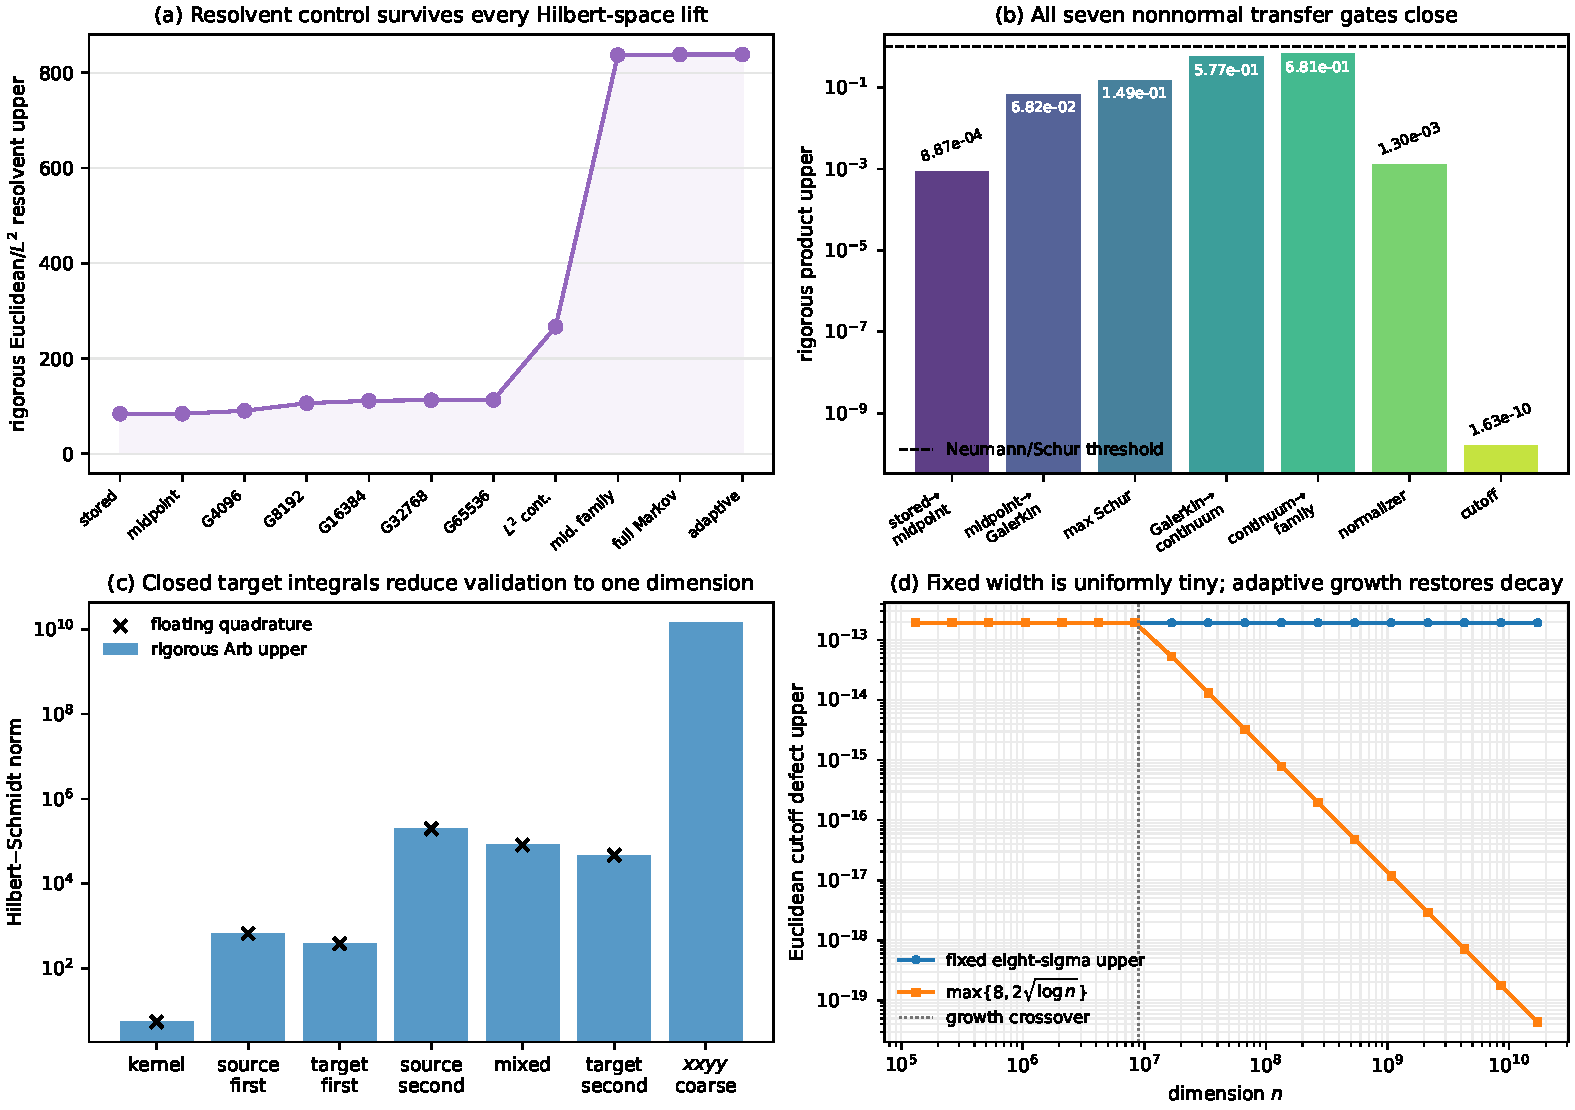
\includegraphics[width=\textwidth]{figures/uniform_euclidean_parity_contour.pdf}
\caption{The Euclidean contour closure.  (a) Rigorous resolvent uppers from
the exact stored matrix through the continuum and the all-grid sparse
family.  (b) All seven nonnormal transfer products are below one.
(c) Closed target integrals and one-dimensional Arb validation give tight
Hilbert--Schmidt constants except for the harmless $h^4$ derivative.
(d) A fixed eight-sigma cutoff stays uniformly tiny in Euclidean norm,
while adaptive growth begins at $n=e^{16}$ and restores decay.}
\label{fig:summary}
\end{figure}

\section{What is closed and what remains}
\label{sec:boundary}

The norm hierarchy can now be stated without ambiguity.
\begin{enumerate}[leftmargin=2em]
 \item \textbf{Continuum parity isolation holds in both \(L^\infty\) and
       \(L^2\).}
       The present Hilbert certificate is independent of dimension-changing
       norm equivalence.
 \item \textbf{The exact full midpoint family has a uniform Euclidean
       contour.}
       From $n=131072$ onward, the full discretely normalized matrices have
       count one and resolvent upper $838.211$.
 \item \textbf{The fixed archived support rule preserves the count.}
       Its Euclidean perturbation is uniformly tiny even though its row
       defect does not vanish.
 \item \textbf{Adaptive support closes the second-order weighted-Riesz
       bridge.}
       The uniform contour and the RH-39 cutoff rate now satisfy every
       premise of the RH-40 perturbation theorem.
 \item \textbf{Exact-real and binary64 families remain distinct.}
       The $4096$ stored binary64 matrix is fully covered by the Grushin and
       Arb ledgers.  The all-dimension theorem concerns the exact-real
       Gaussian formulas; it does not enclose every future transcendental
       binary64 evaluation.
 \item \textbf{Noise is still fixed.}
       The Hilbert derivative constants grow rapidly as $\sigma\downarrow0$.
       No uniform small-noise statement follows from this paper.
\end{enumerate}

The result does not produce a self-adjoint generator, a
$T\log T$ counting law, an arithmetic trace formula, a zeta-zero
identification, or the Riemann hypothesis.  It closes a functional-analytic
discretization gate at one positive noise width.

\section{Archive and reproducibility}
\label{sec:archive}

The archive contains four rigorous ledgers:
\begin{enumerate}[leftmargin=2em]
 \item the exact-stored Euclidean Grushin certificate;
 \item the 224-bit stored-to-midpoint Frobenius bridge;
 \item the 160-bit Hilbert--Schmidt envelope; and
 \item the complete Galerkin, continuum, normalization, and cutoff
       composition certificate.
\end{enumerate}
The floating Gauss--Legendre pilot is archived separately and is never used
as proof.

The complete replay is:
\begin{verbatim}
PYTHONDONTWRITEBYTECODE=1 /root/math/.venv/bin/python \
  -m pytest -q -p no:cacheprovider
PYTHONDONTWRITEBYTECODE=1 /root/math/.venv/bin/python \
  experiments/run_euclidean_grushin_certificate.py
PYTHONDONTWRITEBYTECODE=1 /root/math/.venv/bin/python \
  experiments/build_euclidean_midpoint_bridge.py
PYTHONDONTWRITEBYTECODE=1 /root/math/.venv/bin/python \
  experiments/build_hilbert_envelope_certificate.py
PYTHONDONTWRITEBYTECODE=1 /root/math/.venv/bin/python \
  experiments/build_uniform_euclidean_certificate.py
PYTHONDONTWRITEBYTECODE=1 /root/math/.venv/bin/python \
  experiments/estimate_hilbert_constants.py
MPLBACKEND=Agg PYTHONDONTWRITEBYTECODE=1 \
  /root/math/.venv/bin/python experiments/make_figures.py
latexmk -pdf -interaction=nonstopmode -halt-on-error main.tex
cp main.pdf uniform-euclidean-parity-contour.pdf
PYTHONDONTWRITEBYTECODE=1 /root/math/.venv/bin/python \
  experiments/build_archive.py
PYTHONDONTWRITEBYTECODE=1 /root/math/.venv/bin/python \
  experiments/verify_archive.py
\end{verbatim}

Every consumed cross-paper input, local source, result ledger, figure, and
publication artifact is recorded by SHA-256.

\section{Conclusion}

The continuum parity contour now has a dimension-uniform Hilbert-space
realization.  Exact stored Euclidean residuals start the count, Arb bridges
the binary64 matrix to the analytic midpoint kernel, closed Gaussian moments
validate the Hilbert envelope, and orthogonal Galerkin--Schur continuation
reaches the continuum.  Direct perturbation then controls every sufficiently
fine full and sparse midpoint matrix in the same Euclidean norm.

The fixed eight-sigma window and the adaptive window play different roles.
Fixed width is already uniformly harmless for the spectral count.  Adaptive
growth is what restores convergence of the sparse weighted term to the full
continuum branch.  This distinction closes the final norm condition left by
the weighted-Riesz paper without conflating row and Euclidean topology.

\bibliographystyle{plainnat}
\bibliography{references}

\end{document}
